\documentclass[12pt]{tdtp}
\usepackage{tabularx,colortbl}
\usepackage{multirow}
\usepackage{listings}
\lstset{
	language=VHDL,
basicstyle=\tiny\ttfamily}
\definecolor{light-gray}{gray}{0.96}
\definecolor{pageheading-gray}{gray}{0.2}
\definecolor{dark-gray}{gray}{0.45}
\definecolor{dark-green}{rgb}{0.245,0.121,0.0}

\newcommand{\auteur}{Cedric Lemaitre}
\newcommand{\couriel}{c.lemaitre58@gmail.com}
\newcommand{\promo}{Bachelor in Computer Vision}
\newcommand{\annee}{2016-2017}
\newcommand{\matiere}{Image Processing}

\newcommand{\tdtp}{Labs 1}
\renewcommand{\sujet}{Image transformations}


\begin{document}
\titre

%%%%%%%%%%%%
\Exo

Considering the following image, calculate the size of that image and knowing that the maximum corresponds to a white pixel and the minimum to a black pixel gives the number of bit used for that image.



\begin{figure}[h!]
	\begin{center}
		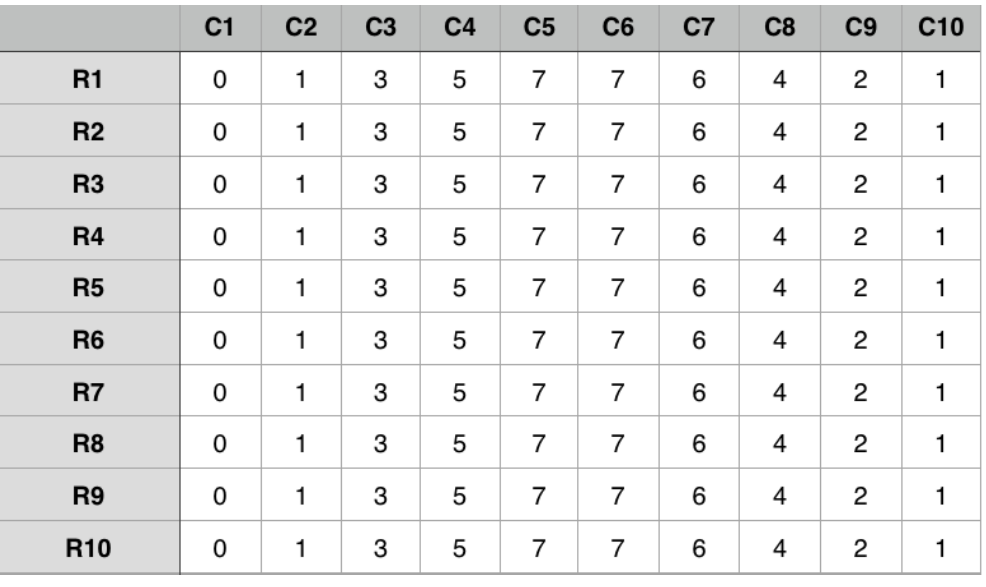
\includegraphics[scale=0.5]{images/I1.png}
		\caption{Input image}
	\end{center}
\end{figure}

%%%%%%%%%%%%
\newpage 
\Exo

Apply that gray level transformation on the previous image.

\begin{figure}[h!]
	\begin{center}
		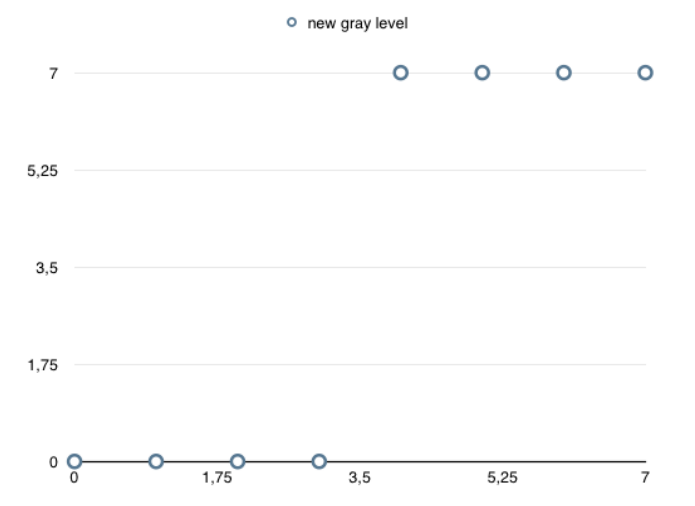
\includegraphics[scale=0.5]{images/I2.png}
		\caption{Input image}
	\end{center}
\end{figure}

Result :



\begin{figure}[h!]
	\begin{center}
		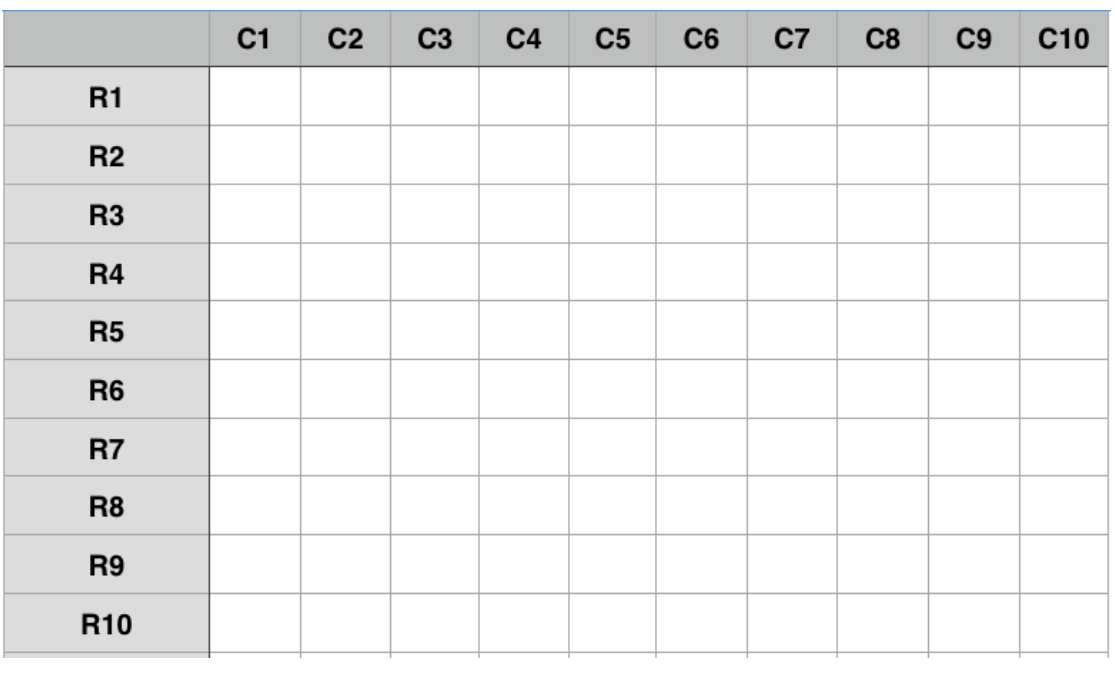
\includegraphics[scale=0.5]{images/I3.png}
		\caption{Input image}
	\end{center}
\end{figure}

%%%%%%%%%%
\newpage 
\Exo


Apply that gray level transformation on the previous image.

\begin{figure}[h!]
	\begin{center}
		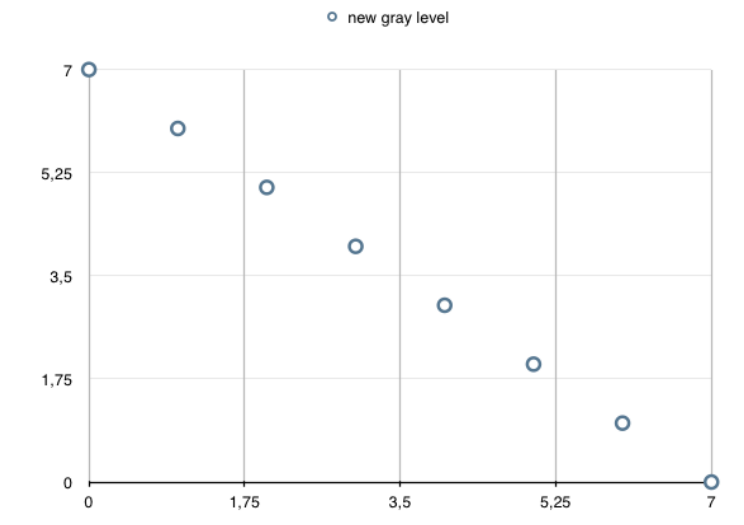
\includegraphics[scale=0.5]{images/I4.png}
		\caption{Input image}
	\end{center}
\end{figure}

Result :



\begin{figure}[h!]
	\begin{center}
		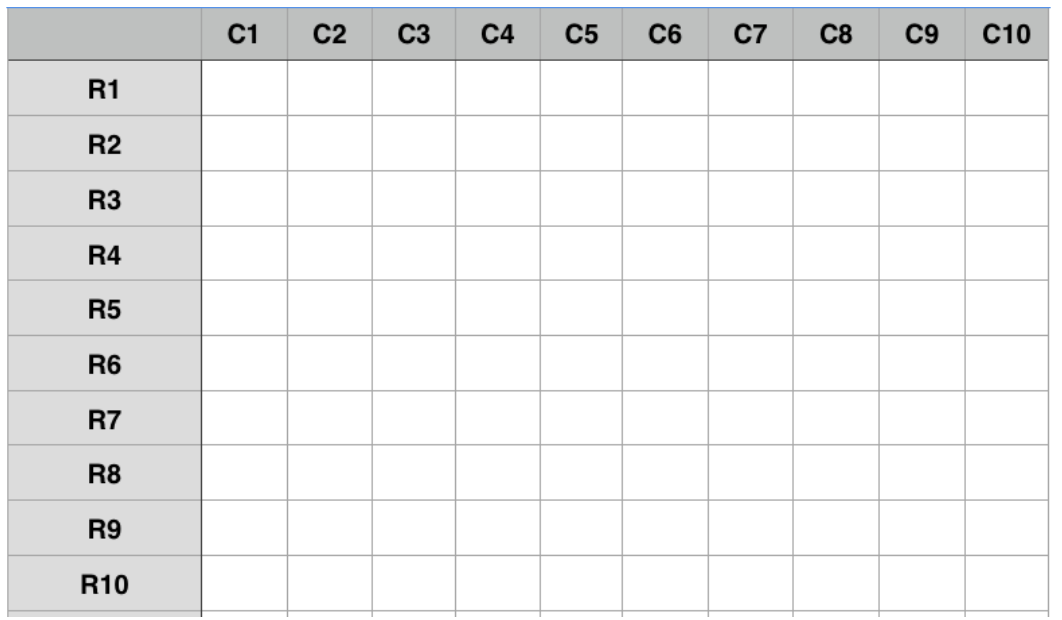
\includegraphics[scale=0.5]{images/I5.png}
		\caption{Input image}
	\end{center}
\end{figure}

%%%%%%%%%%%%%%%%%%%%%%%%%%%%%%%%%%
\newpage
\Exo

Gives the histogram of the first image.\\
Calculate the cumulative distribution function.\\
Apply it to modify the gray levels of the image if we suppose a 8 bits coded image (as input and output).\\
\\

Result


\begin{figure}[h!]
	\begin{center}
		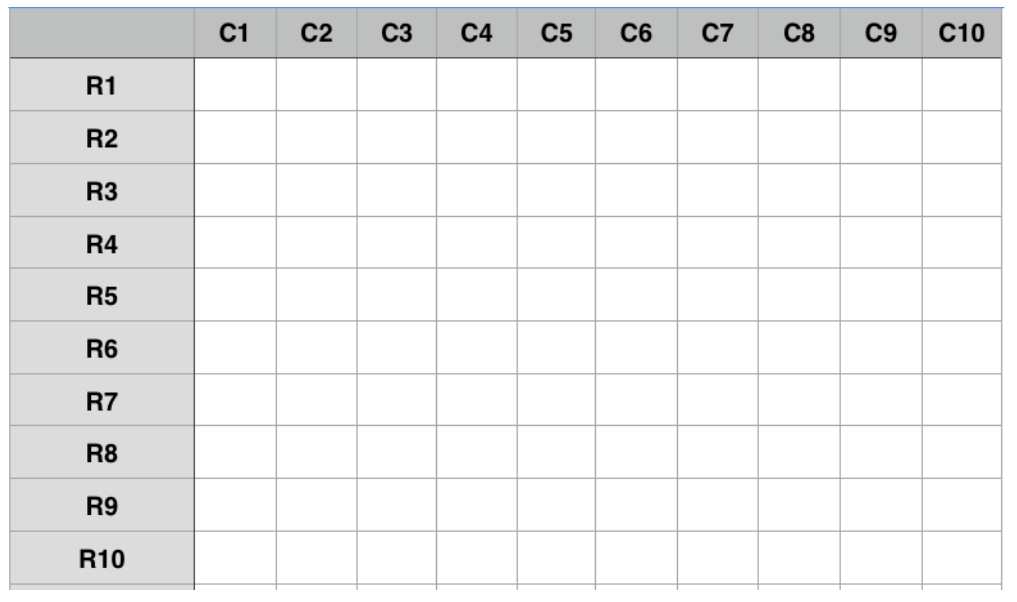
\includegraphics[scale=0.5]{images/I6.png}
		\caption{Input image}
	\end{center}
\end{figure}
\end{document}
